\chapter{并行计算模型的比较}
\label{chap:model-cmp}
\section{并行计算模型综述}
在多年的多核发展中,存在过多种不同的并行计算编程模型,这些编程模型或多或少体现了并行计算以及多核架构开发中软硬件协同的特性,不同的编程模型代表了一类多核架构硬件体系在软件开发领域的抽象,这种抽象的程度以及角度大大影响了使用该模型的开发人员的开发方法和思路,也最终对并行算法的设计产生影响。

在现今使用的多核平台,从普通消费级多核架构,如SMP,到大规模的集群设备,使用最为广泛的几种并行编程模型分别为:
\begin{itemize}
\item 基于分布式内存和消息传递机制的模型,以MPI为代表
\item 基于共享内存的模型,以OpenMP为代表
\item 基于PGAS的模型,以OpenSHMEM为代表
\end{itemize}
在本章中,将对现有的常用的基于CPU的几种并行计算模型从平台模型、内存模型、执行模型以及编程模型4个方面叙述差异。并且最终着眼于OpenSHMEM的特性以及适用范围。
\section{MPI}
在并行计算发展的早期并不存在统一的编程模型,开发过程和资源基本上是以厂商提供的ABI/API为准的,也就是说软件开发直接受限于硬件平台,这种限制严重制约了软件开发的效率和可移植性,这种情况类似于计算机行业发展的早期,开发人员直接操作卡片的方式,对于软硬件开发的分离和统一标准的呼声越来越高。

MPI的标准化工作始于1992年,在威吉尼亚的威廉姆斯堡召开的分布存储环境中消息传递标准的讨论会,由由Dongarra,Hempel,Hey和Walker建议的初始草案于1992年11月推出,并且在1993年2月完成了修订版,即为MPI1.0。由Dongarra,Hempel,Hey和Walker建议的初始草案于1992年11月推出 并在1993年2月完成了修订版,这就是MPI 1.0。为了促进MPI的发展,一个称为MPI论坛的非官方组织应运而生,该论坛对MPI的发展起了重要的作用。

1995年六月推出了MPI的新版本MPI1.1,对原来的MPI作了进一步的修改 完善和扩充,但是当初推出MPI标准时,为了能够使它尽快实现并迅速被接受,许多其它方面的重要但实现起来比较复杂的功能都没有定义,比如并行I/O,当MPI被广为接受之后,扩充并提高MPI功能的要求就越来越迫切了。于是在1997年7月,在原来MPI做了重大扩充的基础上,又增加了MPI的扩充部分MPI-2,MPI-2中并没有对MPI-1做功能上的扩展,而是增加了3个重要的方面:并行I/O, 远程存储访问和动态进程管理。至此,MPI-1和MPI-2已经是一个巨大的多达200余个调用的编程库,并且与Fortran77、C、Fortran99和C++四种语言绑定,涵盖了科学计算领域以及较底层的系统和应用程序对并行编程的需求。

\subsection{内存模型}
严格的说,并行编程模型并不直接定义硬件的结构,也就是说,并不存在某个并行编程模型只能执行在某种类型的平台上的限制,但是实际上,硬件发展的影响对于软件开发的影响直接体现在编程模型对于平台的抽象上,即在使用某个模型时,开发人员将假定程序是运行在这种类型的平台上,而不去考虑真正的底层实现如何。

MPI是消息传递接口(Message Passing Interface)的缩写,并且MPI已经成为这种编程模型的代表和事实标准。消息传递模型在分布式内存并行机上十分容易理解并且高效。
\begin{figure}
\centering
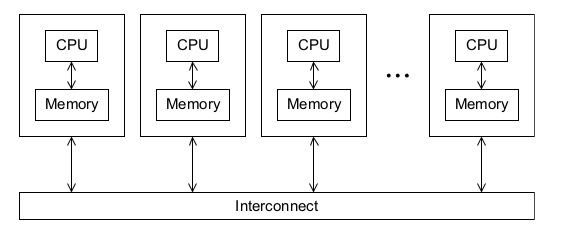
\includegraphics[scale=0.6]{MPI-Distribute_system.png}
\caption{分布式多核系统示意图}\label{fig:dis_sys}
\end{figure}

如图~\ref{fig:dis_sys}所示为分布存储环境下的消息传递的抽象平台,每个计算单元带有自己私有的内存系统,并且通过互联网络
和其他计算单元相连接,两个CPU之间通过传递消息的方式进行通信,这是MPI的核心,即对提供进程之间通信的方式。

假设进程1需要访问进程0的内存内容,则它必须显式的创建一个消息,并且等待进程0接收并且处理该消息,将它需要的内容作为消息内容返回。
\subsection{编程模型}\label{sec:mpi_program}
MPI在程序中通过普通库调用的方式调用,开发者显式的分布任务。MPI-1以及MPI-2库的大小虽然已经很庞大,为开发者提供超过200条调用接口。但是仅仅需要6个调用,就可以写出最简单的MPI程序,这6条调用也是MPI的核心。以一个最简单的Hello world调用这6个函数,如图~\ref{fig:mpi_program}所示说明MPI的编程顺序。源码在附录中。
\begin{figure}
\centering
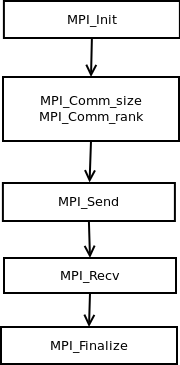
\includegraphics[scale=0.6]{MPI_program.png}
\caption{MPI的编程模型简图}\label{fig:mpi_program}
\end{figure}
如上图所示,开发者需要自己显式的发送和接受数据,并且可以自己定义通信空间(Communication Space),从而组建进程子集进行通信。在MPI\_Send和MPI\_Receive中将目标地址或者源地址作为参数传递,另外需要传递tag以作为数据配对的依据。
\subsection{执行模型}

在图~\ref{fig:mpi_program}中显示的基本的MPI编程模型,编程过程是一个指定串行的过程,然而在MPI程序运行起来之后,具体的说是在MPI\_Init()执行之后,MPI通信空间建立,多个进程将同时运行。如图~\ref{fig:mpi_exe}所示。

\begin{figure}
\centering
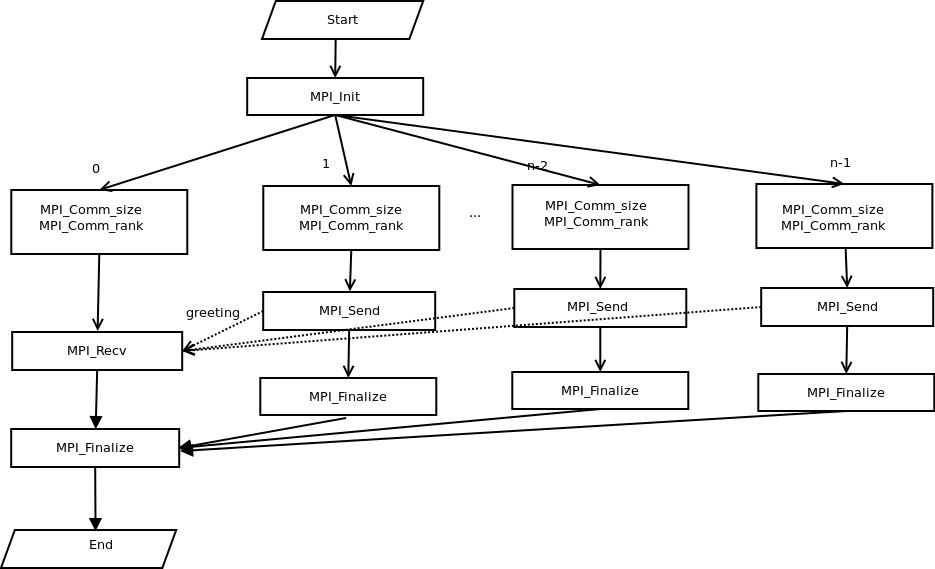
\includegraphics[scale=0.4]{MPI_execute.png}
\caption{MPI程序执行模型}\label{fig:mpi_exe}
\end{figure}

其中参数n为启动的进程数目,n在程序调用时指定。在MPI-1中,启动的进程数目在进程启动后就无法更改,而在MPI-2中增加了动态管理进程的特性。
\section{OpenMP}
OpenMP是共享内存应用的编程接口,它的特性是建立在以往对共享内存并行编程的探索之上。OpenMP被设计为可以适应在一个大范围的SMP架构上实现。随着多核机器以及多线程处理器在市场上的流行,OpenMP可能也会被用于创建运行在单核集群的应用。

就像以前的一些实验性的实现,OpenMP也没有被实现成一种新编程语言,而是被设计成可以通过向串行程序中添加标注的方式达到并行的目的。现有的可以绑定的语言有Fortran, C以及C++,OpenMP描述了如何在多个运行在不同处理器或者核上的线程之间分布任务,并且说明了它们如何访问共享的数据。OpenMP这种插入标注的方式可以让一些现有的串行程序可以在仅需要极少修改的情况下很快的运行在SMP架构上并且享受这种多核架构带来的加速。在实际中,有许多应用中仍存在可观的可以挖掘的并行潜力。

OpenMP的成功归功于一系列的因素,其一是OpenMP对于结构化并行编程的强调,其二是OpenMP易于上手使用,因为OpenMP将大部分的并行任务都交给编译器来完成,并且OpenMP的程序也有比较好的移植性,所以OpenMP程序可以运行在多个不同的平台上。


\subsection{内存模型}
OpenMP仅强调平台模型中所有的内存都是可以共享的,但是并没有要求实际的硬件平台必须是共享内存。
一般的OpenMP应用程序中的平台模型如图~\ref{fig:shared_memo}所示。
\begin{figure}
\centering
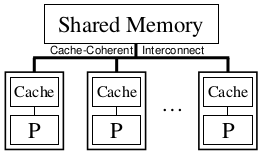
\includegraphics[scale=0.8]{cache-coherent-interconnet.png}
\caption{cache一致的共享内存结构}\label{fig:shared_memo}
\end{figure}

每个处理器(图中的P表示Processor)带有自己的私有缓存,缓存中的数据是不可共享的,需要某种方法保证缓存和内存中内容的一致性,不能出现两个处理器访问同一个内存地址时,因为缓存和内存内容没有同步而出现同一地址两个副本的情况。

内存是全局统一编址的,所有参与的处理器都可以访问,并且多个处理器根据一个地址会访问到同样的内容。很明显,由此引发的最重要的问题就是互斥。这部分将在\ref{sec:shared_exe}部分予以讨论。

另外,在分布式内存环境中,如果要实现OpenMP程序,则需要模拟出共享内存的环境,如图~\ref{fig:dis_shared_memo}所示。实际上,这种平台内存结构和PGAS模型十分相似。
\begin{figure}
\centering 
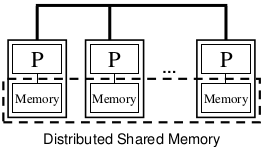
\includegraphics[scale=0.8]{distributed_shared_memory.png}
\caption{分布式环境下的共享内存}\label{fig:dis_shared_memo}
\end{figure}

\subsection{编程模型}
与另一个共享内存的编程模型Pthreads相比,OpenMP的编程方法有一些本质的不同\cite{book:openmp}\cite{book:intro}。Pthreads的方法要求开发者指定每个线程启动之后具体的行动细节,并且要求开发者保证线程动作的可靠性,比如对锁的使用。而OpenMP则仅仅要求开发者在需要并行的地方“说明”需要并行执行的区块,然后将真正决定哪个线程执行哪个或者哪些任务的工作则要交给编译器以及运行时系统来完成。

OpenMP的开发人员也提出了增量式并行过程,即要是用OpenMP进行并行开发,则首先需要创建串行的版本,接着分析串行版本中哪些部分可以并行,就将该部分声明为并行执行区域。这种开发方式很明显对于那些已经存在的串行代码有好处,要将它们重新用MPI或者Pthreads改写,付出的代价要比OpenMP大的多。

OpenMP的并行方式是"基于指令”的。在C/C++中,只需要添加一些预处理命令,就可以让可以辨认这些指令的编译器创建并行程序,而对于不兼容的串行编译器可以直接忽略,并不影响程序的正确性。 

在C/C++中,使用的命令是\emph{\# pragma omp}。其余的形式和串行程序一致,可以参考附录中的示例代码。

\subsection{执行模型}\label{sec:shared_exe}
OpenMP的执行模型是比较典型的fork-join形式。在进入并行区域之前,程序中只有一个线程执行,这个线程可以称为主线程。进入并行区域后主线程立即fork出其他执行线程,可以称为从线程,并且和主线程一起执行计算操作。在计算操作结束后,即到达并行区域的结尾,如图~\ref{fig:openmp_execute},此处会有一个隐式的同步操作,随后所有的线程join到一处,并且结束执行,仅留下主线程继续执行。
\begin{figure}
\centering
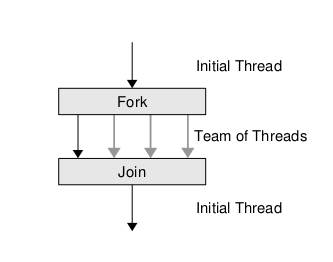
\includegraphics{openmp_execute.png}
\caption{典型的OpenMP的执行模型}\label{fig:openmp_execute}
\end{figure}
\section{OpenSHMEM}
SHMEM是Symmetric Hierarchical MEMory access的简称\cite{book:encyclopedia}。

如在绪论中介绍的,OpenSHMEM是一个基于PGAS模型的编程库的标准化工作,它提供了单端通信(One-sided Communications)的能力。在OpenSHMEM之前,曾经有过多种不同平台和版本的SHMEM实现,但是由于细微的差异,这些SHMEM库都不具有移植性。并且相对于其他同样具有远程内存访问(Remote Memory Access, RMA)语法的支持库,OpenSHMEM也同样具有优势。

现在在科学计算领域使用最多的编程模型和编程方法是MPI,然而MPI使用的是双端通信模型(Two-sided Communications),具体来说,每次通信都必须双方共同的主动参与,发送方需要调用MPI\_Send,接收方则需要调用MPI\_Recv接收,这样才能完成一次通信。这样做的好处是可以在数据通信的同时带来隐式的同步,但在某些场合,这种隐式同步带来的等待开销也是需要被优化掉的。OpenSHMEM提供的单端通信模型就降低了数据传输和和同步之间的耦合度,减少了数据通信的等待时间,并且为RMA提供了可能。

\subsection{内存模型}\label{sec:openshmem_mem}
OpenSHMEM说明文档中说明了数据是如何在内存中存储以及在处理单元(Process Element, PE)之间传递。

在OpenSHMEM中,数据对象可以存储在PE的本地私有内存空间中,也可以存储在PE可以远程访问的内存空间中,存储在本地私有空间中的数据对象只能被拥有该空间的PE所访问,PE可以通过OpenSHMEM调用访问存储在共享区域的数据对象。可以远程访问的数据对象在OpenSHMEM术语中又称为对称对象(Symmetric Objects)。当数据对象在每个PE中都有相同类型和内容的副本时,就被称为对称对象。在C和C++中,可以作为对称对象的可以是静态变量和全局变量 ,因为静态变量和全局变量在编译时就已经确定,所以逻辑上它们应该在所有PE的相同偏移处,并且具有相同的数据类型。如图~\ref{}所示。
\begin{figure}
\centering
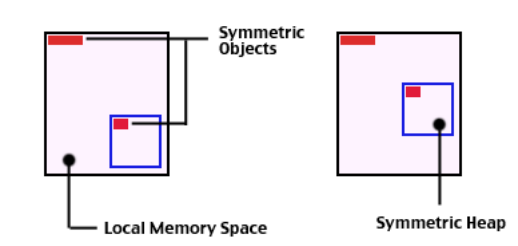
\includegraphics[scale=0.6]{openshmem_symmetric.png}
\caption{OpenSHMEM中对称数据对象示意图}\label{fig:symmetric}
\end{figure}
另外,OpenSHMEM还允许创建动态分配的对称数据对象,和静态的对称数据对象,如全局变量等不同,动态对称数据对象被分配在称为对称堆(Symmetric Heap)的一段特殊的内存区域中,对称堆的分配是在运行时动态决定的,也就是说,对称堆的地址在每个PE上不一定都是一样的。
\subsection{编程模型}
OpenSHMEM采用单指令多数据(Single Process Multiple Data, SPMD)的方式表达并行。

一个OpenSHMEM程序由多个处理器执行,在OpenSHMEM术语中称为PE。和MPI一样,在OpenSHMEM程序开始执行并行任务之前需要先调用start\_pes()进行初始化,如图\ref{fig:openshmem_program}所示。在start\_pes()中执行必要的初始化步骤,比如建立对称堆,组织PE并且将所有PE映射到一个连续数组中,数组下标称为该PE的序号(rank)。rank从0开始,到n-1,n为PE的数目。

接着可以执行数据传输,或者比如广播、归约等操作。可以执行的操作在说明文档\cite{site:openshmem_spec}中一一说明。

和MPI不同的是,OpenSHMEM中并没有规定显式的结束调用,至于如何处理并行程序的结束则是根据实现不同。
\begin{figure}
\centering
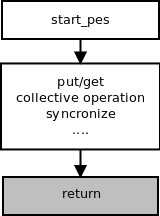
\includegraphics[scale=0.8]{openshmem_program.png}
\caption{OpenSHMEM编程模型}\label{fig:openshmem_program}
\end{figure}
\subsection{执行模型}
因为OpenSHMEM和MPI的调用形式类似,编程方式类似,实际上OpenSHMEM程序的执行顺序和MPI也十分类似。不同之处在于以下两点:
\begin{enumerate}
\item MPI中的数据传输例程需要双端通信,需要收发两方参与,所以在并行部分,Send和Recv总是成对出现,而OpenSHMEM使用的单端读写方式,仅需要主动的一方调用put或者get,无需等待对方的相应;
\item MPI程序的最后需要显式的调用Finalize,作为对并行环境的后续处理,而OpenSHMEM则没有这样的调用。
\end{enumerate}
\section{OpenSHMEM的内容和特性}
在OpenSHMEM说明文档\cite{site:openshmem_spec}中,说明了现有版本的OpenSHMEM提供的所有API。总的说来,可以分为以下6类:
\begin{enumerate}
\item 数据传输操作
\item 原子内存访问操作
\item 集体操作
\item 同步操作
\item 锁操作
\item 环境参数API
\end{enumerate}
从以上可以看出,OpenSHMEM的操作基本是围绕数据进行的,这是因为OpenSHMEM库基本上是针对科学计算等这样以数据为基础的应用设计的,因此OpenSHMEM规定的调用功能范围相对MPI更为精确,可用的调用仅有不到50条,相对于MPI这样庞大的体积,OpenSHMEM则更为灵活小巧。

另外,和MPI、OpenMP以及Pthreads等其他现在主流的编程方法比较,OpenSHMEM强调了以下这样两个特性。
\subsection{PGAS模型}
从前文中对于MPI和OpenMP的介绍中可以看出,MPI基于的硬件模型是分布式存储体系,而OpenMP采用的是共享内存体系,在实际应用中,实际的硬件模型往往是两者的结合,因此在并行计算发展过程中,出现了将MPI和OpenMP混合使用的架构,并且取得了不错的效果\cite{jour:hybrid}。从PGAS模型看来,PGAS模型正是这两种模型的折中,在保留每个核可以唯一访问的私有内存的同时允许共享内存的存在,可以通过调用接口访问远端的内存,也可以以这样的方式通信。实际上,这种模型可能是最接近实际应用的硬件体系抽象,基于该模型的内存模型和通信方式都更直观。

具体到OpenSHMEM中,在\ref{sec:openshmem_mem}小节中可以看到,每个PE都有自己可以访问的私有内存空间,需要通过调用API获取远端共享内存的数据内容,这点和MPI十分类似;而每个PE都可以在任意时刻访问共享内存,无需等待其他PE的应答或者允许,也就是说PE可以通过共享内存快速的通信,这点和共享内存模型也十分契合。
\subsection{单端通信模型}
单端通信模型并非在OpenSHMEM中首次提出。在MPI成为最广泛应用的编程方法的同时,MPI的双端通信的一些弊端也被讨论和改进。因为MPI的每次通信都必须通过类似握手的机制才能完成,在通信未建立时,发送方只能等待,这种同步带来的时间消耗在数据量十分大的情况下可以看作比较小的消耗,但是对于数据量较小但是发送较频繁的情况,这种同步消耗称为比较明显的需要优化的点,即如何将数据传输和同步解耦合。

在OpenSHMEM的介绍中,可以看到OpenSHMEM的数据通信方式都是单端的,一个PE的操作无需等待另一个PE的应答就可以单方面的完成。OpenSHMEM的基本操作是远程内存访问(RMA),提供的基本方法remote put/get也是每个支持RMA的编程方法都具有的。RMA可以算作单端通信的一个例子。要完成RMA,一定是单端的,因为无法预期在何时会有远程访问,因此除了不断轮询这种耗时的方法外,很难将RMA实现为双端的。

在并行计算发展的很长一段时间里,网络硬件的发展十分缓慢,并行体系在设计时需要考虑对网络的兼容和在有限带宽下提高性能。然而,在过去的几年中,网络通信硬件的飞速发展为底层通信带来了几个新的概念,比如零拷贝(Zero-Copy),OS bypass\cite{jour:cci}等等。一个著名的新一代网络硬件的例子是Infiniband,在Infiniband中,硬件集成了对RDMA的支持,这代表了新一代网络发展的方向,然而在MPI和OpenMP中,并没有表现出对这种新特性的支持。因此,可以认为,对于单端通信模型的支持是OpenSHMEM的一大亮点,对于RDMA以及尤其对小数据量友好的单端通信模型是近年来PGAS模型语言重新获得关注的主要原因。